\documentclass[11pt,a4paper]{article}

% ---------- Paket ----------
\usepackage[a4paper,margin=2.2cm]{geometry}
\usepackage[utf8]{inputenc}
\usepackage[T1]{fontenc}
\usepackage{amsmath,amssymb,mathtools,bm}
\usepackage{xcolor}
\usepackage{booktabs}
\usepackage{array}
\usepackage{longtable}
\usepackage{enumitem}
\usepackage{tcolorbox}
\tcbuselibrary{skins,breakable}
\usepackage{listings}
\usepackage{hyperref}
\usepackage{titlesec}
\usepackage{fancyhdr}
\usepackage{parskip}
\usepackage{tikz}
\usetikzlibrary{positioning,arrows.meta}

% ---------- Warna ----------
\definecolor{navy}{HTML}{0B3D91}
\definecolor{steel}{HTML}{1a5276}
\definecolor{noteBg}{HTML}{FFF6E5}
\definecolor{noteBd}{HTML}{F0C36D}
\definecolor{okBg}{HTML}{EAF7EE}
\definecolor{okBd}{HTML}{8FCB9E}
\definecolor{codeBg}{HTML}{1E1E1E}
\definecolor{codeFg}{HTML}{D4D4D4}
\definecolor{formulaBg}{HTML}{F2F5FA}
\definecolor{formulaBd}{HTML}{B9C6DA}

% ---------- Heading style ----------
\titleformat{\section}{\large\bfseries\color{navy}}{\thesection}{0.6em}{}
\titleformat{\subsection}{\normalsize\bfseries\color{steel}}{\thesubsection}{0.6em}{}
\titleformat{\subsubsection}{\normalsize\bfseries\color{black!70}}{\thesubsubsection}{0.6em}{}
\titlespacing*{\section}{0pt}{1.4em}{0.6em}
\titlespacing*{\subsection}{0pt}{1.0em}{0.4em}

\pagestyle{fancy}
\fancyhf{}
\renewcommand{\headrulewidth}{0.4pt}
\lhead{\small\textcolor{black!60}{Penjelasan Lengkap MLP 3-4-1 — Sidang Skripsi}}
\rhead{\small\textcolor{black!60}{\thepage}}

% ---------- Kotak rumus ----------
\newtcolorbox{formulabox}{
  breakable, enhanced, colback=formulaBg, colframe=formulaBd,
  boxrule=0.6pt, arc=1.5mm, left=6pt, right=6pt, top=6pt, bottom=6pt
}
\newtcolorbox{notebox}{
  breakable, enhanced, colback=noteBg, colframe=noteBd,
  boxrule=0.6pt, arc=1.5mm, left=6pt, right=6pt, top=6pt, bottom=6pt,
  title={\textbf{Catatan}}, coltitle=black, fonttitle=\bfseries,
  attach title to upper
}
\newtcolorbox{verdictbox}{
  breakable, enhanced, colback=okBg, colframe=okBd,
  boxrule=0.6pt, arc=1.5mm, left=6pt, right=6pt, top=6pt, bottom=6pt
}

% ---------- Code listing style ----------
\lstdefinestyle{cstyle}{
  backgroundcolor=\color{codeBg},
  basicstyle=\ttfamily\footnotesize\color{codeFg},
  keywordstyle=\color{cyan},
  commentstyle=\color{green!60!black},
  numberstyle=\tiny\color{gray},
  breaklines=true,
  frame=none,
  xleftmargin=8pt, xrightmargin=8pt,
  aboveskip=8pt, belowskip=8pt,
  showstringspaces=false
}
\lstset{style=cstyle}

\hypersetup{
  colorlinks=true, linkcolor=navy, urlcolor=navy, citecolor=navy,
  pdftitle={Penjelasan Lengkap MLP 3-4-1 untuk Sidang Skripsi},
  pdfauthor={Yoel}
}

\newcommand{\tanhp}{\operatorname{tanh}}

\title{\color{navy}\textbf{Penjelasan Lengkap Alur Kerja\\MLP Pressure Controller 3-4-1}}
\author{\large Dari Data Mentah, Normalisasi, \emph{Forward} \& \emph{Backward Propagation},\\
hingga Implementasi Bobot ke Mikrokontroler STM32}
\date{Dokumen pendamping sidang skripsi --- disusun berdasarkan notebook\\
\texttt{training\_mlp\_3input\_closedloop.ipynb}\\
(Training MLP Pressure Controller 3-4-1, Data Closed-Loop, 14 Juni 2026)}

\begin{document}

\maketitle

\begin{abstract}
\noindent Dokumen ini menjelaskan secara runtut dan matematis seluruh alur kerja model
\emph{Multilayer Perceptron} (MLP) berarsitektur 3-4-1 yang dipakai sebagai pengontrol
tekanan pompa: mulai dari sumber data CSV, rekayasa fitur, normalisasi, arsitektur
jaringan, penurunan rumus \emph{forward pass}, fungsi \emph{loss}, penurunan rumus
\emph{backpropagation} secara manual, pemilihan \emph{optimizer} dan \emph{learning rate},
evaluasi model (termasuk analisis \emph{overfitting}/\emph{underfitting} dengan angka aktual
hasil training), hingga cara ke-21 parameter bobot dipindahkan menjadi array bahasa C dan
dieksekusi di STM32. Semua angka numerik pada dokumen ini diambil langsung dari output
eksekusi notebook (bukan ilustrasi), sehingga dapat dipertanggungjawabkan saat sidang.
\end{abstract}

\tableofcontents
\newpage

% =====================================================================
\section{Gambaran Umum \& Tujuan Sistem}

Sistem yang dibangun adalah sebuah \textbf{pengontrol tekanan pompa berbasis Jaringan
Saraf Tiruan} (\emph{Artificial Neural Network}, ANN). Alih-alih memakai kontroler klasik
seperti PID yang parameternya diturunkan secara analitis, jaringan ini \textbf{belajar
meniru cara operator manusia mengambil keputusan} menaikkan/menurunkan \emph{duty cycle}
PWM pompa berdasarkan data historis (disebut \emph{behavior cloning}).

Model menerima \textbf{3 input}:
\begin{itemize}[nosep]
  \item $\mathrm{error}$ --- selisih \emph{setpoint} dan tekanan aktual,
  \item $\Delta\mathrm{error}$ --- laju perubahan error (menangkap tren/percepatan),
  \item $\mathrm{duty}_t$ --- posisi \emph{duty cycle} aktuator saat ini,
\end{itemize}
dan mengeluarkan \textbf{1 output}: $\Delta\mathrm{Duty}$, yaitu \emph{perubahan} duty
cycle yang harus dilakukan --- bukan nilai duty absolut. Nilai duty untuk langkah
berikutnya diperoleh dengan:

\begin{formulabox}
\[
  \mathrm{duty}_{k+1} \;=\; \operatorname{clamp}\!\big(\mathrm{duty}_k + \Delta\mathrm{Duty}_{\text{pred}},\; 70,\; 95\big)
\]
\end{formulabox}

Desain ini disengaja: dengan memprediksi \emph{perubahan} (bukan nilai absolut), model
tidak bisa hanya ``menyalin'' nilai duty sebelumnya sebagai jawaban aman (jebakan yang
pernah terjadi pada notebook versi lama, dibahas di Bagian~\ref{sec:featureeng}). Model
dipaksa benar-benar mempelajari \textbf{hubungan sebab-akibat} antara kondisi tekanan dan
aksi koreksi yang tepat.

% =====================================================================
\section{Kenapa MLP? (Posisi MLP di Antara Jenis-Jenis ANN)}

``\emph{Neural network}'' adalah istilah payung. Model yang dipakai di sini adalah
\textbf{ANN jenis MLP (\emph{Multilayer Perceptron})}, disebut juga \emph{feedforward
fully-connected network}:

\begin{center}
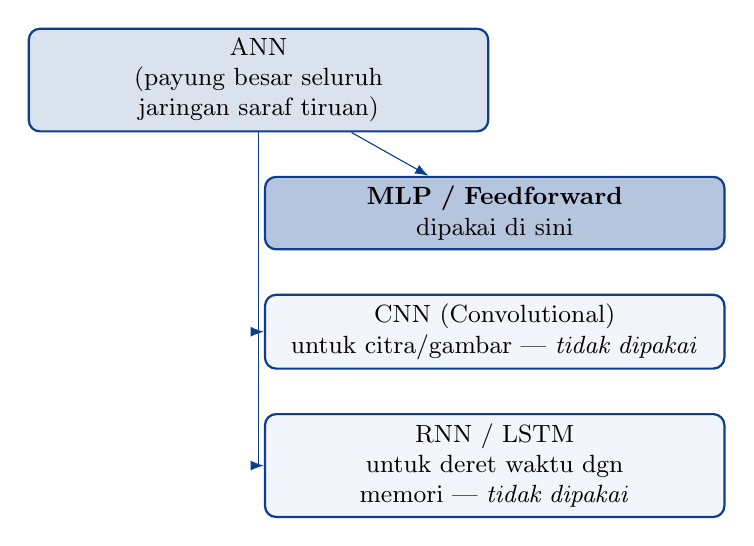
\begin{tikzpicture}[
  node distance=0.55cm and 2.2cm,
  every node/.style={font=\small},
  box/.style={rectangle, rounded corners, draw=navy, thick, fill=formulaBg, align=center, minimum height=0.9cm, text width=5.6cm}
]
\node[box, fill=navy!15] (ann) {ANN\\(payung besar seluruh jaringan saraf tiruan)};
\node[box, below=of ann, xshift=3.0cm, fill=navy!30] (mlp) {\textbf{MLP / Feedforward}\\dipakai di sini};
\node[box, below=of mlp] (cnn) {CNN (Convolutional)\\untuk citra/gambar --- \emph{tidak dipakai}};
\node[box, below=of cnn] (rnn) {RNN / LSTM\\untuk deret waktu dgn memori --- \emph{tidak dipakai}};
\draw[-{Latex}, navy] (ann) -- (mlp);
\draw[-{Latex}, navy] (ann.south) |- (cnn.west);
\draw[-{Latex}, navy] (ann.south) |- (rnn.west);
\end{tikzpicture}
\end{center}

\textbf{Bukan CNN} --- CNN dirancang untuk citra (mendeteksi pola spasial dengan filter
konvolusi); data pada kasus ini bukan gambar. \textbf{Bukan RNN} --- RNN memiliki memori
antar-waktu (\emph{recurrent state}); pada kasus ini, informasi tren waktu dimasukkan
secara eksplisit lewat fitur $\Delta\mathrm{error}$, sehingga MLP sederhana sudah cukup
menangkap dinamika sistem tanpa kompleksitas RNN.

\textbf{Alasan pemilihan MLP untuk kasus ini:}
\begin{enumerate}[nosep]
  \item Hubungan input--output bersifat statis per langkah keputusan (bukan sekuens panjang
  yang perlu diingat).
  \item Jumlah data terbatas (ratusan baris) sehingga arsitektur kecil lebih cocok dan
  tidak membutuhkan data sebanyak CNN/RNN.
  \item MLP kecil (21 parameter) sangat ringan untuk dieksekusi \emph{real-time} di
  mikrokontroler STM32 dengan memori terbatas.
\end{enumerate}

% =====================================================================
\section{Arsitektur Jaringan 3-4-1 dan Jumlah Parameter}

Notasi ``3-4-1'' berarti: 3 neuron input, 4 neuron \emph{hidden} (satu lapis
tersembunyi), 1 neuron output.

\begin{center}
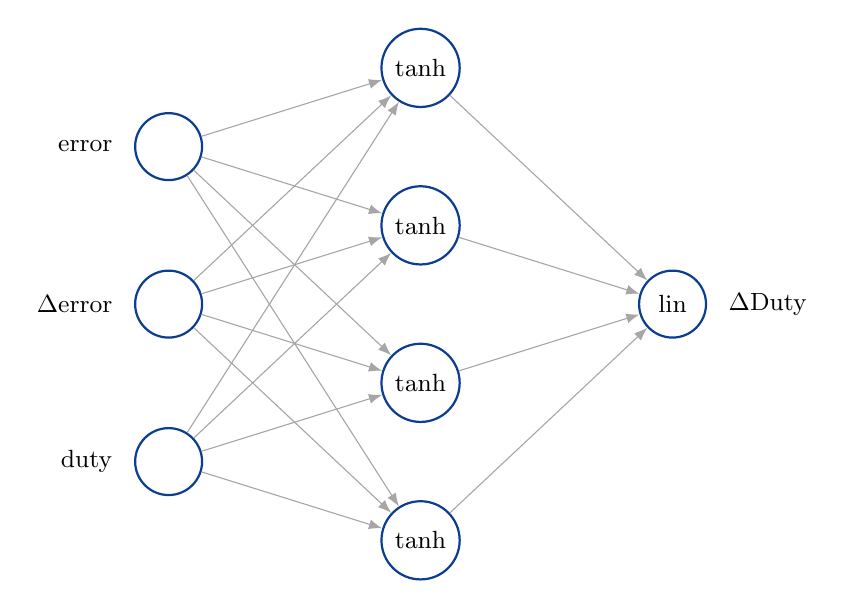
\begin{tikzpicture}[
  node distance=1.1cm and 2.4cm,
  neuron/.style={circle, draw=navy, thick, minimum size=0.85cm, font=\small},
  lbl/.style={font=\small}
]
% input layer
\node[neuron] (i1) at (0,2.0) {};
\node[neuron] (i2) at (0,0.0) {};
\node[neuron] (i3) at (0,-2.0) {};
\node[lbl, left=0.15cm of i1] {$\mathrm{error}$};
\node[lbl, left=0.15cm of i2] {$\Delta\mathrm{error}$};
\node[lbl, left=0.15cm of i3] {$\mathrm{duty}$};

% hidden layer
\node[neuron] (h1) at (3.2,3.0) {$\tanh$};
\node[neuron] (h2) at (3.2,1.0) {$\tanh$};
\node[neuron] (h3) at (3.2,-1.0) {$\tanh$};
\node[neuron] (h4) at (3.2,-3.0) {$\tanh$};

% output layer
\node[neuron] (o1) at (6.4,0.0) {lin};
\node[lbl, right=0.15cm of o1] {$\Delta\mathrm{Duty}$};

\foreach \i in {i1,i2,i3}
  \foreach \h in {h1,h2,h3,h4}
    \draw[-{Latex}, gray!70] (\i) -- (\h);
\foreach \h in {h1,h2,h3,h4}
  \draw[-{Latex}, gray!70] (\h) -- (o1);
\end{tikzpicture}
\end{center}

Setiap garis pada diagram adalah satu \textbf{bobot} (\emph{weight}); setiap neuron
(selain input) memiliki satu \textbf{bias}. Jumlah parameter yang benar-benar
``dipelajari'' saat training:

\begin{center}
\begin{tabular}{@{}l l r@{}}
\toprule
\textbf{Layer} & \textbf{Perhitungan} & \textbf{Jumlah} \\
\midrule
Input $\to$ Hidden ($W_1,\,b_1$) & $3 \times 4$ bobot $+\ 4$ bias & $12+4=16$ \\
Hidden $\to$ Output ($W_2,\,b_2$) & $4 \times 1$ bobot $+\ 1$ bias & $4+1=5$ \\
\midrule
\textbf{TOTAL} & & \textbf{21 parameter} \\
\bottomrule
\end{tabular}
\end{center}

Model sekecil ini (21 angka \emph{float}) hanya membutuhkan puluhan--ratusan sampel data
untuk dilatih dengan stabil, dan saat inferensi di STM32 hanya perlu $<21$
perkalian--penjumlahan $+\ 4$ evaluasi $\tanh$ --- jauh lebih ringan dibanding CNN/RNN.

% =====================================================================
\section{Dari CSV ke Dataset Latih: Rekayasa Fitur}
\label{sec:featureeng}

\subsection{Penggabungan File \& Penomoran Episode Global}

Data terekam sebagai 12 file CSV terpisah, total 4.035 baris mentah. Setiap file memiliki
\texttt{episode\_id} yang mulai dari 1 lagi (tidak unik antarfile). Jika langsung
digabung, dua episode berbeda dari file berbeda bisa dianggap satu episode yang sama,
sehingga perhitungan selisih ($\Delta$) antarbaris akan ``menyambung'' dua kejadian yang
sebenarnya tidak berhubungan (transisi palsu).

Solusinya: setiap pasangan \texttt{(file, episode\_id)} diberi identitas baru
\texttt{global\_episode} yang unik. Hasil aktual: \textbf{16 episode global} dari 12 file;
baris korup (misalnya catatan manual seperti ``3 keran lupa'') dibuang otomatis lewat
\texttt{dropna}.

\subsection{Hanya Memakai Baris Keputusan}

Sensor mencatat data secara kontinu, tetapi \emph{controller} hanya benar-benar
\emph{mengambil keputusan} tiap 3 detik (baris dengan \texttt{is\_decision == 1}). Dari
4.035 baris mentah, hanya \textbf{469 baris keputusan} yang relevan untuk dilatih --- baris
lain dibuang karena tidak merepresentasikan momen pengambilan aksi.

\subsection{Rumus Tiga Fitur Input dan Satu Target}

\begin{center}
\begin{tabular}{@{}p{2.6cm} p{5.6cm} p{6.4cm}@{}}
\toprule
\textbf{Kolom} & \textbf{Rumus} & \textbf{Peran} \\
\midrule
$\mathrm{error}$ & $\mathrm{setpoint\_bar} - \mathrm{pressure\_bar}$ & Input 1 --- seberapa jauh dari target \\
$\mathrm{d\_error}$ & $\mathrm{error}_k - \mathrm{error}_{k-1}$ per \texttt{global\_episode} & Input 2 --- tren/kecepatan perubahan error \\
$\mathrm{duty\_percent}$ & apa adanya (posisi aktuator) & Input 3 --- kondisi aktuator saat ini \\
$\mathrm{delta\_duty}$ & $\mathrm{duty}_{k+1} - \mathrm{duty}_{k}$ per \texttt{global\_episode} & \textbf{TARGET} --- aksi koreksi berikutnya yang benar-benar dilakukan manusia \\
\bottomrule
\end{tabular}
\end{center}

Operasi selisih dilakukan \textbf{per \texttt{global\_episode}} (memakai
\texttt{groupby}) agar tidak menyambung antarepisode yang tidak berhubungan. Baris
terakhir tiap episode otomatis dibuang karena targetnya kosong (tidak ada ``baris
berikutnya'' untuk dihitung selisihnya). Setelah proses ini: \textbf{453 baris siap latih}
(dari 469 baris keputusan).

\begin{notebox}
Karena target adalah $\mathrm{delta\_duty}$ = aksi yang benar-benar diambil operator,
model belajar meniru kebijakan kontrol manusia --- bukan sekadar meniru sinyal masa lalu.
Ini penting: pada notebook versi lama, target sempat didefinisikan sebagai nilai duty
absolut baris berikutnya, yang secara numerik sangat mirip dengan input $\mathrm{duty}_t$
itu sendiri --- sehingga model ``curang'' cukup meng-copy input menjadi output dan tampak
seolah sangat akurat ($R^2 = 0{,}98$ \emph{palsu}). Formulasi $\mathrm{delta\_duty}$ pada
notebook ini menutup celah tersebut.
\end{notebox}

\subsection{Sebaran Target (Bukti Data Tidak Trivial)}

\begin{center}
\begin{tabular}{@{}l r r@{}}
\toprule
\textbf{Kategori aksi} & \textbf{Jumlah baris} & \textbf{Persentase} \\
\midrule
Naik ($\Delta\mathrm{Duty} > 0$)  & 161 & 35,5\% \\
Turun ($\Delta\mathrm{Duty} < 0$) & 91  & 20,1\% \\
Tahan ($\Delta\mathrm{Duty} = 0$) & 201 & 44,4\% \\
\bottomrule
\end{tabular}
\end{center}

Nilai target hanya berupa bilangan bulat $\{-3,-2,-1,0,1,2,3\}$ (\%) sesuai granularitas
\emph{step} keputusan manusia. Sebarannya cukup berimbang, dan korelasi $\mathrm{error}$
vs $\Delta\mathrm{Duty}$ bersifat sedang--kuat namun \textbf{bukan $1{,}0$} --- artinya
hubungan bersifat non-linear (itulah pekerjaan yang harus dipelajari MLP, bukan sekadar
garis lurus).

% =====================================================================
\section{Normalisasi Input (StandardScaler)}
\label{sec:norm}

Ketiga fitur input memiliki skala yang sangat berbeda: $\mathrm{error}$ berkisar di angka
$0{,}1$-an (bar), sedangkan $\mathrm{duty\_percent}$ berkisar $65$--$95$ (\%). Jika
dibiarkan tanpa penyesuaian, neuron akan bias memberi bobot besar hanya karena skala
angkanya besar (bukan karena informasinya lebih penting), dan proses training menjadi
tidak stabil / lambat konvergen. Solusinya: \textbf{StandardScaler}, yang mengubah setiap
fitur menjadi rata-rata 0 dan simpangan baku (\emph{std}) 1:

\begin{formulabox}
\[
  x'_i \;=\; \frac{x_i - \mu_i}{\sigma_i}, \qquad i = 1,2,3
\]
\end{formulabox}

dengan $\mu_i$ (mean) dan $\sigma_i$ (std) dihitung \textbf{hanya dari data Train} (agar
informasi data Val/Test tidak ``bocor'' ke proses penskalaan), lalu nilai yang sama
dipakai untuk mentransformasi Val, Test, dan nanti data baru saat inferensi di STM32.
Nilai aktual hasil \texttt{fit} pada dataset ini (tersimpan di ekspor firmware, Bagian
\ref{sec:stm32}):

\begin{center}
\begin{tabular}{@{}l r r@{}}
\toprule
\textbf{Fitur} & $\mu$ (mean) & $\sigma$ (std/scale) \\
\midrule
$\mathrm{error}$        & $-0{,}01586624$ & $0{,}11593238$ \\
$\mathrm{d\_error}$     & $\phantom{-}0{,}00100443$  & $0{,}06163191$ \\
$\mathrm{duty\_percent}$ & $82{,}27215190$ & $7{,}13180498$ \\
\bottomrule
\end{tabular}
\end{center}

\textbf{Contoh numerik:} bila $\mathrm{error} = 0{,}05$ bar, maka
\[
  x'_1 = \frac{0{,}05 - (-0{,}01587)}{0{,}11593} \approx 0{,}569
\]
Angka $0{,}569$ inilah yang sebenarnya masuk ke neuron hidden, bukan $0{,}05$ mentah.

\begin{notebox}
Parameter $\mu$ dan $\sigma$ ini \textbf{BUKAN} bobot jaringan saraf, tetapi statistik
data --- namun tetap wajib disalin ke STM32 dan diterapkan pada input mentah
\emph{sebelum} masuk ke perhitungan $W_1$, karena bobot $W_1/W_2$ dilatih dengan asumsi
input sudah dinormalisasi seperti ini.
\end{notebox}

% =====================================================================
\section{Pembagian Data: Train / Validation / Test}
\label{sec:split}

Dari 453 baris siap latih, data dibagi acak (\emph{shuffle}) dengan proporsi kurang lebih
$70\% : 10\% : 20\%$, menghasilkan pembagian aktual:

\begin{center}
\begin{tabular}{@{}l r p{7.4cm}@{}}
\toprule
\textbf{Subset} & \textbf{Jumlah baris} & \textbf{Fungsi} \\
\midrule
Train      & 316 & Dipakai langsung untuk menyetel (mengubah) bobot $W_1,b_1,W_2,b_2$ \\
Validation & 46  & Memantau kapan model mulai \emph{overfitting}; TIDAK dipakai menyetel bobot \\
Test       & 91  & ``Ujian akhir'' --- data yang sama sekali tak dilihat model selama training \\
\bottomrule
\end{tabular}
\end{center}

\begin{notebox}
Pembagian ini dilakukan \emph{per baris keputusan} secara acak, bukan \emph{per episode}.
Ada kemungkinan baris-baris dari episode yang sama tersebar ke lebih dari satu subset
(Train dan Test), yang berpotensi membuat metrik Test sedikit lebih optimis dibanding jika
diuji dengan episode yang benar-benar baru sepenuhnya (dibahas lebih dalam di Bagian
\ref{sec:overfit}).
\end{notebox}

% =====================================================================
\section{\emph{Forward Propagation} --- Penurunan Rumus Lengkap}
\label{sec:forward}

\emph{Forward pass} adalah proses menghitung output ($\Delta\mathrm{Duty}$) dari input
mentah. Diberikan input $x=[\mathrm{error},\Delta\mathrm{error},\mathrm{duty}]$ yang sudah
dinormalisasi (Bagian~\ref{sec:norm}) menjadi $x' = [x'_1,x'_2,x'_3]$, perhitungan
berjalan dalam dua tahap.

\subsection{Tahap 1 --- Lapisan \emph{Hidden} (4 neuron, aktivasi $\tanh$)}

Untuk setiap neuron hidden $j = 1,\dots,4$, hitung jumlah berbobot (\emph{pre-activation})
lalu terapkan fungsi aktivasi:

\begin{formulabox}
\begin{align}
  z^{(1)}_j &= b^{(1)}_j + \sum_{i=1}^{3} x'_i \, W^{(1)}_{ij} \label{eq:z1}\\
  h_j &= \tanh\!\big(z^{(1)}_j\big) \label{eq:h}
\end{align}
\end{formulabox}

$W_1$ berukuran $3\times4$ (satu kolom per neuron hidden, satu baris per input); $b_1$
adalah vektor bias sepanjang 4. Hasilnya $h=[h_1,h_2,h_3,h_4]$, masing-masing bernilai di
rentang $(-1,+1)$ karena $\tanh$.

\subsection{Tahap 2 --- Lapisan Output (1 neuron, LINEAR / tanpa aktivasi)}

\begin{formulabox}
\[
  \Delta\mathrm{Duty} \;=\; \hat{y} \;=\; b^{(2)} + \sum_{j=1}^{4} h_j \, W^{(2)}_j
\]
\end{formulabox}

Output \textbf{sengaja dibuat linear} (tanpa $\tanh$/\emph{sigmoid}) karena
$\Delta\mathrm{Duty}$ bukan probabilitas atau nilai terbatas $0$--$1$; ia perlu bisa
bernilai negatif (menurunkan duty), nol (menahan), maupun positif (menaikkan) tanpa
dibatasi rentang buatan. Membatasi output dengan fungsi aktivasi non-linear di sini justru
akan merusak kemampuan model memprediksi besaran koreksi yang proporsional.

\begin{verdictbox}
Ringkas: \emph{forward pass} hanyalah \textbf{perkalian--penjumlahan $+$ satu fungsi
non-linear ($\tanh$) di tengah}. Inilah sebabnya inferensi MLP sangat murah secara
komputasi dan cocok dijalankan berulang-ulang secara \emph{real-time} di MCU kelas STM32.
\end{verdictbox}

% =====================================================================
\section{Fungsi Aktivasi $\tanh$ --- Kenapa Dipilih \& Turunannya}
\label{sec:tanh}

Tanpa fungsi aktivasi non-linear di lapisan hidden, seluruh jaringan (betapa pun banyak
lapisannya) secara matematis akan runtuh menjadi satu \textbf{fungsi linear tunggal} ---
karena komposisi dari fungsi-fungsi linear tetaplah linear:
\[
  f_2\big(f_1(x)\big) = W_2\big(W_1 x + b_1\big) + b_2 = \underbrace{(W_2 W_1)}_{W'} x + \underbrace{(W_2 b_1 + b_2)}_{b'}
\]
Tanpa non-linearitas, MLP hanya akan sekuat regresi linear biasa dan tidak bisa
mempelajari hubungan $\mathrm{error}\to\Delta\mathrm{Duty}$ yang melengkung (non-linear)
seperti ditunjukkan oleh data (korelasi sedang, bukan $1{,}0$).

Fungsi $\tanh$ (tangen hiperbolik) didefinisikan sebagai:

\begin{formulabox}
\[
  \tanh(z) \;=\; \frac{e^{z}-e^{-z}}{e^{z}+e^{-z}}, \qquad \text{rentang keluaran: } (-1,+1)
\]
\end{formulabox}

Turunannya (dipakai saat \emph{backpropagation}, Bagian~\ref{sec:backprop}):

\begin{formulabox}
\[
  \frac{d}{dz}\big[\tanh(z)\big] \;=\; 1-\tanh^2(z) \;=\; 1-h^2
\]
\end{formulabox}

\subsection{Alasan Pemilihan $\tanh$ (Dibanding ReLU atau Sigmoid)}

\begin{itemize}[nosep]
  \item Keluaran $\tanh$ \textbf{zero-centered} (simetris di sekitar 0, rentang
  $-1..+1$), cocok karena fitur $\mathrm{error}$ dan $\Delta\mathrm{error}$ juga bisa
  bernilai negatif maupun positif secara natural --- representasi internal jaringan jadi
  selaras dengan sifat fisis sinyal kontrol (deviasi dua arah dari \emph{setpoint}).
  \item Untuk jaringan sekecil ini (1 \emph{hidden layer}, 4 neuron), $\tanh$ tidak
  mengalami masalah \emph{vanishing gradient} separah pada jaringan yang sangat dalam,
  sehingga aman dipakai.
  \item Dibanding ReLU: ReLU cenderung menghasilkan output kontrol yang ``patah-patah''
  (\emph{piecewise linear} dengan sudut tajam) untuk sistem kontrol kontinu bertekanan;
  $\tanh$ menghasilkan permukaan keputusan yang lebih mulus (\emph{smooth}), sesuai
  karakter sinyal tekanan yang kontinu.
  \item Sigmoid (rentang $0..1$) kurang cocok karena tidak \emph{zero-centered} --- akan
  memperlambat konvergensi \emph{optimizer} dibanding $\tanh$ untuk kasus regresi
  bernilai dua arah seperti ini.
\end{itemize}

% =====================================================================
\section{Fungsi \emph{Loss} (MSE) --- Ukuran Kesalahan Model}
\label{sec:loss}

Selama training, model perlu tahu ``seberapa salah'' prediksinya agar bisa memperbaiki
diri. Ukuran ini disebut \textbf{loss}. Notebook memakai \textbf{Mean Squared Error
(MSE)}, rata-rata kuadrat selisih antara prediksi dan target sebenarnya, dihitung atas
$N$ sampel data:

\begin{formulabox}
\[
  L \;=\; \mathrm{MSE} \;=\; \frac{1}{N}\sum_{n=1}^{N}\big(\hat{y}_n - y_n\big)^2
\]
\end{formulabox}

dengan $\hat{y}_n = \Delta\mathrm{Duty}$ hasil prediksi model untuk sampel ke-$n$, dan
$y_n = \Delta\mathrm{Duty}$ sebenarnya (label dari data manusia). Kuadrat dipakai karena
dua alasan: (1) menghilangkan tanda negatif sehingga error positif dan negatif tidak
saling meniadakan, (2) menghukum kesalahan besar jauh lebih keras daripada kesalahan
kecil (error $2\times$ lipat $\to$ kontribusi ke loss $4\times$ lipat), mendorong model
menghindari prediksi yang sangat meleset.

Untuk kebutuhan turunan gradien per-sampel (Bagian~\ref{sec:backprop}), lebih mudah
memakai bentuk per-sampel dengan faktor $\tfrac12$ (agar turunannya bersih, konvensi umum
di literatur \emph{backpropagation}):

\begin{formulabox}
\[
  L_n \;=\; \tfrac{1}{2}\big(\hat{y}_n - y_n\big)^2
\]
\end{formulabox}

% =====================================================================
\section{\emph{Backward Propagation} --- Penurunan Rumus Gradien Manual}
\label{sec:backprop}

\emph{Backpropagation} adalah proses menghitung \textbf{seberapa besar dan ke arah mana}
setiap satu dari 21 parameter ($W_1,b_1,W_2,b_2$) harus diubah agar loss $L$ mengecil.
Caranya: menerapkan \textbf{aturan rantai} (\emph{chain rule}) turunan, merambat mundur
dari output ke input. Di \texttt{scikit-learn} (\texttt{MLPRegressor}) proses ini
otomatis, tetapi untuk sidang penting bisa diturunkan sendiri secara manual seperti
berikut, memakai notasi Bagian~\ref{sec:forward} (satu sampel data).

\subsection{Langkah 1 --- Gradien di Lapisan Output (linear)}

\begin{formulabox}
\begin{align}
  \delta_{\text{out}} \;=\; \frac{\partial L}{\partial \hat{y}} &= \hat{y}-y \label{eq:dout}\\[4pt]
  \frac{\partial L}{\partial W^{(2)}_j} &= \delta_{\text{out}}\cdot h_j, \qquad j=1,\dots,4 \\
  \frac{\partial L}{\partial b^{(2)}} &= \delta_{\text{out}}
\end{align}
\end{formulabox}

Karena aktivasi output linear ($f(z)=z,\ f'(z)=1$), turunannya sederhana: gradien
terhadap bobot $W^{(2)}_j$ adalah error output ($\delta_{\text{out}}$) dikalikan aktivasi
hidden yang bersangkutan ($h_j$) --- intuisinya: neuron hidden yang ``menyala'' besar
($h_j$ besar) dan ikut andil dalam kesalahan, akan disalahkan lebih besar dan bobotnya
diubah lebih banyak.

\subsection{Langkah 2 --- Merambatkan Error ke Lapisan \emph{Hidden}}

\begin{formulabox}
\begin{align}
  \frac{\partial L}{\partial h_j} &= \delta_{\text{out}}\cdot W^{(2)}_j
  \qquad\text{(seberapa besar $h_j$ menyumbang error output)}\\[4pt]
  \delta^{(1)}_j \;=\; \frac{\partial L}{\partial z^{(1)}_j}
  &= \underbrace{\big(\delta_{\text{out}}\cdot W^{(2)}_j\big)}_{\partial L/\partial h_j}\cdot
  \underbrace{\big(1-h_j^{2}\big)}_{\tanh'(z^{(1)}_j)} \label{eq:delta1}
\end{align}
\end{formulabox}

Di sinilah turunan $\tanh$ dari Bagian~\ref{sec:tanh} dipakai: $(1-h_j^2)$. Perhatikan
bahwa jika $h_j$ mendekati $\pm1$ (neuron ``jenuh''/saturasi), maka $(1-h_j^2)$ mendekati
$0$ --- gradien yang mengalir ke bobot sebelumnya jadi sangat kecil. Ini fenomena
\emph{vanishing gradient} pada $\tanh$; untuk jaringan sedangkal ini (1 \emph{hidden
layer}) dampaknya masih terkendali, sehingga $\tanh$ tetap aman dipakai (lihat
Bagian~\ref{sec:tanh}).

\subsection{Langkah 3 --- Gradien di Lapisan Input $\to$ \emph{Hidden}}

\begin{formulabox}
\begin{align}
  \frac{\partial L}{\partial W^{(1)}_{ij}} &= \delta^{(1)}_j \cdot x'_i, \qquad i=1,\dots,3,\ j=1,\dots,4 \\
  \frac{\partial L}{\partial b^{(1)}_j} &= \delta^{(1)}_j
\end{align}
\end{formulabox}

Untuk satu \emph{batch} berisi banyak sampel, gradien di atas dirata-ratakan (atau
dijumlahkan lalu dibagi $N$) di seluruh sampel dalam \emph{batch} tersebut sebelum
dipakai memperbarui bobot.

\subsection{Langkah 4 --- Pembaruan Bobot (\emph{Gradient Descent} Dasar)}

\begin{formulabox}
\begin{align}
  W &\;\leftarrow\; W \;-\; \eta\,\frac{\partial L}{\partial W} \\
  b &\;\leftarrow\; b \;-\; \eta\,\frac{\partial L}{\partial b}
\end{align}
\end{formulabox}

dengan $\eta$ (\emph{eta}) adalah \textbf{learning rate} --- seberapa besar langkah
perubahan bobot setiap kali update (dibahas rinci di Bagian~\ref{sec:optimizer}). Proses
Langkah 1--4 ini diulang berkali-kali (banyak \emph{epoch}, satu epoch = satu kali melihat
seluruh data Train) sampai loss stabil kecil atau berhenti membaik.

\begin{verdictbox}
\textbf{Ringkasan intuisi \emph{backprop} untuk dijelaskan lisan di sidang:} ``Error di
output dihitung dulu (selisih prediksi$-$target), lalu error itu ditelusuri mundur ---
dibagi-bagikan ke tiap neuron hidden sesuai kontribusinya (lewat bobot $W_2$), dikalikan
dengan seberapa sensitif neuron itu terhadap perubahan (turunan $\tanh$), lalu dipakai
untuk menghitung arah koreksi tiap bobot $W_1$. Semua bobot diperbarui sedikit demi
sedikit ke arah yang menurunkan loss.''
\end{verdictbox}

% =====================================================================
\section{\emph{Optimizer} \& \emph{Learning Rate}}
\label{sec:optimizer}

Notebook memakai \textbf{dua \emph{solver} berbeda untuk dua tujuan berbeda} --- poin ini
penting dijelaskan dengan tepat saat sidang agar tidak terkesan tidak konsisten:

\begin{center}
\begin{tabular}{@{}p{2.6cm} p{3.6cm} p{7.9cm}@{}}
\toprule
\textbf{Solver} & \textbf{Dipakai untuk} & \textbf{Karakteristik} \\
\midrule
\texttt{lbfgs}\newline (Limited-memory BFGS) & Model FINAL yang dievaluasi (Bagian~\ref{sec:eval}) \& diekspor ke STM32 (Bagian~\ref{sec:stm32}) &
Optimizer \emph{quasi-Newton}, memakai pendekatan informasi kelengkungan (Hessian) fungsi
loss. Sangat efisien \& cepat konvergen untuk dataset \textbf{kecil} (ratusan sampel,
puluhan parameter) seperti kasus ini. Tidak membutuhkan \emph{learning rate} manual
(\emph{self-tuning} secara internal) dan tidak mengekspos loss per-epoch. \\
\addlinespace
\texttt{adam}\newline (Adaptive Moment Estimation) & HANYA untuk menggambar kurva loss per-epoch (Bagian~\ref{sec:overfit}) --- model paralel, terpisah dari model final &
Optimizer berbasis \emph{gradient descent} dengan momentum \& \emph{learning rate}
adaptif per-parameter. Membutuhkan \texttt{learning\_rate\_init} (diset $0{,}02$) dan
cocok dilatih bertahap (\texttt{partial\_fit}) sehingga loss tiap epoch bisa direkam \&
diplot. \\
\bottomrule
\end{tabular}
\end{center}

\subsection{Kenapa \texttt{lbfgs} Dipilih sebagai Model Final (bukan \texttt{adam})?}

Dokumentasi resmi \texttt{scikit-learn} (dan pengalaman umum) menyatakan \texttt{lbfgs}
dapat konvergen lebih cepat dan memberi hasil lebih baik untuk dataset kecil dibanding
\emph{solver} berbasis \emph{gradient descent} stokastik seperti \texttt{adam}/\texttt{sgd}.
Karena dataset di sini hanya 316 baris Train dengan 21 parameter (rasio data:parameter
$\approx 15{:}1$, tergolong kecil), \texttt{lbfgs} adalah pilihan yang lebih sesuai dan
lebih stabil dibanding menyetel \emph{learning rate} manual pada \texttt{adam}.

\subsection{Apa Itu \emph{Learning Rate} dan Kenapa Nilainya Penting?}

\emph{Learning rate} ($\eta$) mengendalikan besar langkah setiap pembaruan bobot (lihat
rumus Langkah 4, Bagian~\ref{sec:backprop}). Analogi: menuruni lembah loss dengan mata
tertutup --- $\eta$ adalah panjang setiap langkah kaki.

\begin{itemize}[nosep]
  \item \textbf{$\eta$ terlalu besar}: langkah terlalu lebar, bisa melompati titik
  minimum loss, training tidak stabil / loss berosilasi bahkan naik-turun tak menentu,
  bisa gagal konvergen.
  \item \textbf{$\eta$ terlalu kecil}: langkah terlalu pendek, training menjadi sangat
  lambat, dan berisiko ``tersangkut'' di titik datar/\emph{local minimum} yang bukan
  solusi terbaik dalam jumlah epoch terbatas.
  \item Pada eksperimen kurva loss (\emph{solver} \texttt{adam}), nilai
  $\eta_{\text{init}} = 0{,}02$ dipilih sebagai kompromi: cukup besar untuk konvergen
  dalam ratusan epoch (bukan ribuan), tapi tidak terlalu besar sehingga val loss tetap
  turun mulus (tidak berosilasi) sebelum akhirnya menyentuh titik terbaiknya di epoch 259
  (lihat Bagian~\ref{sec:overfit}).
\end{itemize}

\textbf{Epoch} = satu kali jaringan melihat/melewati seluruh data Train sekali penuh.
Semakin banyak epoch, semakin banyak kesempatan bobot diperbarui --- tetapi epoch
berlebihan tanpa kontrol adalah salah satu penyebab utama \emph{overfitting} (dibahas di
Bagian~\ref{sec:overfit}).

% =====================================================================
\section{Regularisasi ($\alpha$) --- Mencegah \emph{Overfitting}}
\label{sec:reg}

Selain arsitektur kecil dan skema Train/Val/Test, notebook menambahkan satu mekanisme
lagi untuk menahan \emph{overfitting}: \textbf{regularisasi L2}, diaktifkan lewat
parameter $\alpha = 10^{-3}$ pada \texttt{MLPRegressor}. Regularisasi L2 menambahkan
``biaya'' ke fungsi loss yang dilatih, sebanding dengan besarnya kuadrat semua bobot:

\begin{formulabox}
\[
  L_{\text{total}} \;=\; \mathrm{MSE} \;+\; \alpha \sum \Big( \big(W^{(1)}\big)^2 + \big(W^{(2)}\big)^2 \Big)
\]
\end{formulabox}

Efeknya: model ``dihukum'' jika bobot menjadi sangat besar, sehingga \emph{optimizer}
cenderung memilih solusi dengan bobot yang lebih kecil dan halus --- mengurangi risiko
model ``menghafal'' titik-titik data latih secara ekstrem (yang biasanya butuh bobot
besar/tajam). Nilai $\alpha=0{,}001$ tergolong regularisasi ringan (tidak terlalu
memaksa, mengingat modelnya sudah sangat kecil dengan hanya 21 parameter, sehingga risiko
overfit dari besarnya kapasitas model itu sendiri memang relatif rendah).

% =====================================================================
\section{Evaluasi Model: MAE, RMSE, $R^2$}
\label{sec:eval}

Tiga metrik dipakai untuk menilai akurasi model pada data Train, Validation, dan Test:

\begin{formulabox}
\begin{align}
  \mathrm{MAE} &= \frac{1}{N}\sum_{n=1}^{N} \big|\hat{y}_n - y_n\big|
  &&\text{rata-rata besar kesalahan (\% duty)} \\
  \mathrm{RMSE} &= \sqrt{\frac{1}{N}\sum_{n=1}^{N} \big(\hat{y}_n - y_n\big)^2}
  &&\text{sama seperti MAE, tapi hukum error besar lebih keras} \\
  R^2 &= 1 - \frac{\sum_n (\hat{y}_n - y_n)^2}{\sum_n (y_n - \bar{y})^2}
  &&\text{proporsi variasi target yang dijelaskan model}
\end{align}
\end{formulabox}

$R^2=1$ berarti prediksi sempurna; $R^2=0$ berarti model sama baiknya dengan sekadar
menebak rata-rata target setiap saat; $R^2$ negatif berarti model lebih buruk daripada
tebakan rata-rata itu sendiri. Hasil aktual pada model final (\emph{pipeline}
\texttt{StandardScaler} + \texttt{MLPRegressor} \emph{solver} \texttt{lbfgs}):

\begin{center}
\begin{tabular}{@{}l r r r@{}}
\toprule
\textbf{Subset} & \textbf{RMSE (\%)} & \textbf{MAE (\%)} & $\bm{R^2}$ \\
\midrule
Train (316 baris)      & 0,4171 & 0,3110 & 0,9324 \\
Validation (46 baris)  & 0,5409 & 0,3341 & 0,8817 \\
Test (91 baris)        & 0,4629 & 0,3287 & 0,9152 \\
\bottomrule
\end{tabular}
\end{center}

Interpretasi: pada data Test yang \emph{sama sekali belum pernah dilihat model selama
training}, rata-rata kesalahan prediksi hanya $\pm0{,}33\%$ duty cycle (MAE), dan model
mampu menjelaskan $91{,}5\%$ variasi keputusan $\Delta\mathrm{Duty}$ manusia
($R^2=0{,}9152$). Ini adalah performa yang tergolong \textbf{baik} untuk kasus
\emph{behavior cloning} dengan data lapangan yang bising (\emph{noisy}, sebab manusia
tidak selalu konsisten mengambil keputusan).

% =====================================================================
\section{Analisis \emph{OVERFITTING} vs \emph{UNDERFITTING} (Jawaban Jujur)}
\label{sec:overfit}

Ini adalah bagian yang paling sering ditanyakan penguji sidang: \emph{``Bagaimana Anda
tahu model Anda tidak overfit atau underfit?''} Berikut penjelasan konsep dan
penerapannya pada angka aktual hasil training notebook ini --- dijawab apa adanya,
termasuk kelemahannya.

\subsection{Definisi \& Cara Membaca Kurva Loss}

\begin{center}
\begin{tabular}{@{}p{5.2cm} p{5.0cm} p{2.9cm}@{}}
\toprule
\textbf{Pola pada kurva Loss (Train vs Val)} & \textbf{Artinya} & \textbf{Diagnosis} \\
\midrule
Train loss turun, Val loss ikut turun dan tetap dekat dengan Train loss &
Model belajar pola umum yang berlaku juga di data baru & \textbf{FIT BAIK} \\
\addlinespace
Train loss turun terus hingga sangat kecil, tapi Val loss berhenti turun lalu justru
\emph{NAIK} kembali setelah suatu epoch &
Model mulai ``menghafal'' data latih (termasuk \emph{noise}-nya) & \textbf{OVERFITTING} \\
\addlinespace
Train loss \emph{dan} Val loss sama-sama masih tinggi / tidak turun signifikan meski
epoch ditambah &
Model terlalu sederhana atau belum cukup belajar bahkan di data yang dilihatnya sendiri &
\textbf{UNDERFITTING} \\
\bottomrule
\end{tabular}
\end{center}

Prinsip singkatnya: \textbf{\emph{overfitting} dilihat dari GAP} (jarak) antara performa
Train dan Val/Test --- Val jauh lebih buruk dari Train. \textbf{\emph{Underfitting}
dilihat dari LEVEL} --- keduanya sama-sama buruk.

\subsection{Penerapan pada Angka Aktual Notebook}

\textbf{(a) Dari tabel metrik final (Bagian~\ref{sec:eval}, model \texttt{lbfgs}):} gap
$R^2$ Train ($0{,}9324$) vs Test ($0{,}9152$) hanya sekitar
\[
  \Delta R^2 = 0{,}9324 - 0{,}9152 = 0{,}0172
\]
sangat kecil. Gap RMSE Train ($0{,}417$) vs Test ($0{,}463$) juga tipis. Jika model
overfit berat, pola khasnya adalah Train $R^2$ sangat tinggi mendekati 1 (hafal)
sementara Test $R^2$ jatuh jauh (misalnya di bawah $0{,}5$). Pola itu \textbf{tidak
terjadi} di sini.

\textbf{(b) Validation ($R^2=0{,}8817$) justru sedikit lebih rendah dari Test
($R^2=0{,}9152$)} --- ini agak tidak biasa (biasanya Val cenderung setara/lebih optimis
dari Test), namun paling mungkin disebabkan oleh \textbf{ukuran subset Validation yang
sangat kecil (hanya 46 baris)}. Pada sampel sekecil ini, satu-dua titik ``sulit''
(episode dengan keputusan manusia yang kurang konsisten) bisa menggeser $R^2$ cukup jauh
murni karena variansi pengambilan sampel (\emph{sampling variance}), bukan indikasi
sistematis model gagal generalisasi.

\textbf{(c) Dari kurva loss} (Bagian~\ref{sec:optimizer}, eksperimen \emph{solver}
\texttt{adam} + \emph{early stopping}), log training mencatat:

\begin{formulabox}
\centering
\texttt{Stop di epoch 509\ \ |\ \ best val MSE 0,1543 @ epoch 259}
\end{formulabox}

Skema \emph{early stopping} memakai \emph{patience} $=250$ epoch: training baru
dihentikan jika 250 epoch berturut-turut val loss tidak membaik lagi dari titik
terbaiknya. Karena training berhenti di epoch $259+250=509$, ini artinya \textbf{setelah
epoch $\approx259$, val loss berhenti membaik} --- itu adalah sinyal klasik \emph{mulai
terjadi overfitting ringan} jika training diteruskan tanpa batas. Namun karena
\emph{checkpoint} ``terbaik'' yang diambil adalah tepat di epoch 259 (sebelum tren
memburuk berlanjut), mekanisme \emph{early stopping} sudah bekerja dengan benar untuk
mencegah \emph{overfitting} tersebut menular ke model yang dipakai.

\begin{notebox}
Model pada eksperimen kurva loss ini (\emph{solver} \texttt{adam}, \emph{early-stopped})
adalah \textbf{model paralel/terpisah} --- arsitektur dan datanya sama, tetapi bobot
akhirnya \underline{berbeda} dari model final yang dievaluasi di Bagian~\ref{sec:eval}
dan diekspor ke STM32 di Bagian~\ref{sec:stm32} (yang memakai \emph{solver}
\texttt{lbfgs}). Alasannya: \texttt{lbfgs} adalah metode \emph{quasi-Newton} yang tidak
berjalan per-epoch seperti \emph{gradient descent} sehingga tidak bisa direkam kurva
loss-nya secara alami; \emph{solver} \texttt{adam} dipakai khusus sebagai ``kaca
pembesar'' tambahan untuk melihat pola belajar model, bukan untuk menghasilkan bobot
final.
\end{notebox}

\subsection{Satu Risiko Metodologi yang Perlu Diungkap Secara Jujur}

Pembagian Train/Val/Test (Bagian~\ref{sec:split}) dilakukan secara acak \textbf{per baris
keputusan}, bukan \textbf{per episode}. Karena baris-baris keputusan dalam satu episode
yang sama saling berkorelasi secara temporal (fitur $\Delta\mathrm{error}$ dihitung dari
baris sebelumnya dalam episode yang sama), ada kemungkinan sebagian baris dari satu
episode masuk ke Train sementara baris lain dari episode yang sama masuk ke Test. Ini
berpotensi menimbulkan sedikit \textbf{kebocoran informasi antarsubset} (\emph{data
leakage}), yang bisa membuat metrik Test ($R^2=0{,}9152$) \emph{sedikit lebih optimis}
daripada performa sesungguhnya jika model diuji pada episode yang benar-benar 100\% baru
dan belum pernah ``terlihat'' sama sekali polanya oleh model. Uji yang lebih ketat untuk
memvalidasi ini adalah skema \emph{leave-one-episode-out cross-validation} (satu episode
utuh disisihkan penuh sebagai Test, tidak ada barisnya sama sekali yang masuk Train).

\subsection{Verdict / Kesimpulan Jujur}

\begin{verdictbox}
\textbf{Tidak underfit} --- $R^2$ di atas $0{,}88$ pada seluruh subset (Train/Val/Test),
jauh melampaui kedua \emph{baseline} pembanding (Bagian~\ref{sec:baseline}), menandakan
model sudah cukup kompleks untuk menangkap pola non-linear pada data ini.

\textbf{Tidak overfit secara nyata pada model final} --- gap Train vs Test $R^2$ sangat
tipis ($<0{,}02$), sebuah tanda generalisasi yang sehat, ditopang oleh arsitektur kecil
(21 parameter), regularisasi L2 ($\alpha$), dan skema Train/Val/Test yang konsisten.

\textbf{Ada indikasi \emph{overfitting} ringan bila training diteruskan tanpa batas} ---
terlihat dari kurva loss eksperimen (val loss berhenti membaik setelah epoch
$\approx259$) --- namun ini adalah perilaku training yang \emph{normal dan sudah
diantisipasi dengan benar} lewat mekanisme \emph{early stopping}, bukan cacat pada model
final.

\textbf{Titik lemah paling jujur untuk diakui secara proaktif:} ukuran Validation set
yang kecil (46 baris) dan skema \emph{split} berbasis baris (bukan berbasis episode)
membuat angka Test berpotensi sedikit bias optimis. Ini sebaiknya disampaikan sebagai
\emph{saran pengembangan lanjutan} (\emph{future work}) --- misalnya evaluasi tambahan
dengan \emph{leave-one-episode-out} --- bukan disembunyikan, karena kesadaran akan
keterbatasan metodologi justru memperkuat kredibilitas ilmiah di mata penguji.
\end{verdictbox}

% =====================================================================
\section{Perbandingan dengan \emph{Baseline} (Bukti Model Berguna)}
\label{sec:baseline}

\emph{Baseline} adalah model pembanding yang sangat sederhana, gunanya membuktikan bahwa
MLP benar-benar memberi nilai tambah dibanding tebakan naif. Dua \emph{baseline} diuji
pada data Test yang sama:

\begin{center}
\begin{tabular}{@{}p{3.5cm} r r r p{4.0cm}@{}}
\toprule
\textbf{Model} & \textbf{RMSE} & \textbf{MAE} & $\bm{R^2}$ & \textbf{Interpretasi} \\
\midrule
MLP 3-4-1 & 0,4629 & 0,3287 & 0,9152 & Model yang diusulkan \\
\addlinespace
\emph{Baseline} $\Delta\mathrm{Duty}=0$ (diam saja) & 1,5967 & 1,1209 & $-0{,}0094$ &
$R^2$ negatif $\to$ lebih buruk dari sekadar menebak rata-rata \\
\addlinespace
\emph{Baseline} Proporsional ($\Delta\mathrm{Duty}=k\cdot\mathrm{error}$, $k=10{,}49$
hasil \emph{least-squares}) & 0,9996 & 0,7402 & 0,6044 & Kontroler-P linear sederhana;
masih jauh di bawah MLP \\
\bottomrule
\end{tabular}
\end{center}

Gain proporsional $k$ dicari lewat regresi \emph{least-squares} sederhana pada data
Train:
\[
  k \;=\; \frac{\sum_n x_{1,n}\, y_n}{\sum_n x_{1,n}^2} \;=\; 10{,}49
\]

MLP mengungguli kedua \emph{baseline} secara signifikan: dibanding \emph{baseline} ``diam
saja'', error MLP (RMSE $0{,}46$) jauh lebih kecil dari \emph{baseline} diam (RMSE
$1{,}60$). Dibanding kontroler Proporsional linear terbaik yang mungkin dibuat dari data
ini (RMSE $1{,}00$, $R^2=0{,}60$), MLP masih jauh lebih baik (RMSE $0{,}46$,
$R^2=0{,}92$). Ini adalah \textbf{bukti kuantitatif} bahwa MLP menangkap pola
\underline{non-linear} dalam pengambilan keputusan manusia yang tidak bisa
direpresentasikan oleh satu garis lurus ($k\cdot\mathrm{error}$) saja --- inilah nilai
tambah nyata dari pendekatan \emph{neural network} dibanding kontroler klasik
proporsional.

% =====================================================================
\section{Simulasi \emph{Closed-Loop} (Model sebagai \emph{Controller})}

Evaluasi pada Bagian~\ref{sec:eval} hanya menguji akurasi prediksi $\Delta\mathrm{Duty}$
satu langkah (``\emph{open-loop}''). Untuk menguji apakah model layak dipakai sebagai
\emph{controller} sungguhan, dilakukan simulasi \textbf{closed-loop}: dimulai dari duty
awal episode (data lapangan yang punya jumlah baris keputusan terbanyak), lalu pada tiap
langkah $k$:

\begin{enumerate}[nosep]
  \item Hitung $\mathrm{error}_k$ \& $\Delta\mathrm{error}_k$ dari tekanan AKTUAL yang
  terekam (dipakai sebagai representasi gangguan/\emph{plant} sungguhan, bukan hasil
  simulasi tekanan model).
  \item Model memprediksi $\Delta\mathrm{Duty}_k$ dari
  $[\mathrm{error}_k,\Delta\mathrm{error}_k,\mathrm{duty}_{\text{sim},k-1}]$.
  \item $\mathrm{duty}_{\text{sim},k} = \operatorname{clamp}(\mathrm{duty}_{\text{sim},k-1}+\Delta\mathrm{Duty}_k,\,70,\,95)$.
  \item Ulangi untuk seluruh langkah dalam episode.
\end{enumerate}

Hasilnya dibandingkan dengan rekaman duty asli yang dilakukan manusia pada episode
tersebut. Jika kurva duty hasil simulasi model mengikuti pola kurva duty manusia dengan
baik, itu bukti model mampu berperilaku sebagai \emph{controller} yang konsisten
sepanjang waktu --- bukan hanya akurat pada prediksi satu langkah yang terisolasi.

% =====================================================================
\section{Ekspor Bobot ke STM32 --- Matriks C \& \emph{Forward Pass} \emph{Embedded}}
\label{sec:stm32}

Setelah training selesai, seluruh 21 parameter (\emph{mean}/\emph{scale} \emph{scaler} +
$W_1,b_1,W_2,b_2$) dikeluarkan sebagai \emph{array} C konstan (\texttt{static const
float}) yang siap disalin langsung ke \emph{source code} \emph{firmware} STM32 --- tidak
perlu \emph{library machine learning} apa pun di sisi mikrokontroler, cukup \emph{array}
angka dan beberapa baris kode C. Berikut nilai aktual yang dihasilkan notebook untuk
model final:

\begin{lstlisting}[language=C]
/* === MLP 3-4-1 (input: error, d_error, duty) === */
static const float scaler_mean[3]  = { -0.01586624f,  0.00100443f, 82.27215190f };
static const float scaler_scale[3] = {  0.11593238f,  0.06163191f,  7.13180498f };

static const float W1[3][4] = {
    { -1.15757672f,  1.71712945f,  -3.65813410f, -16.90999678f },
    {  0.00773297f,  0.17402844f,  -3.60776505f,   7.44927295f },
    {  0.92057488f,  0.77042528f, -11.97423637f,  10.49031145f }
};
static const float B1[4] = { 0.50083114f, -0.39519265f, -22.83592021f, -7.20119188f };

static const float W2[4] = { -1.36458051f, 1.70422781f, 0.99562945f, -0.30379082f };
static const float B2[1] = { 1.25671514f };
\end{lstlisting}

\textbf{Kode \emph{forward pass} di \emph{firmware} C} (dijalankan tiap 3 detik di
STM32), sengaja ditulis identik secara matematis dengan rumus Bagian~\ref{sec:forward}:

\begin{lstlisting}[language=C]
float in[3] = { error, d_error, duty };

/* langkah 1: normalisasi (StandardScaler), WAJIB sebelum masuk W1 */
for (i = 0; i < 3; i++)
    in[i] = (in[i] - scaler_mean[i]) / scaler_scale[i];

/* langkah 2: lapisan hidden, 4 neuron, aktivasi tanh  ==>  z1_j, h_j (Persamaan 3-4) */
for (j = 0; j < 4; j++) {
    float s = B1[j];
    for (i = 0; i < 3; i++) s += in[i] * W1[i][j];
    h[j] = tanhf(s);
}

/* langkah 3: lapisan output, 1 neuron, LINEAR (tanpa aktivasi) */
float dd = B2[0];
for (j = 0; j < 4; j++) dd += h[j] * W2[j];

/* langkah 4: terapkan ke duty, batasi ke rentang aman aktuator */
duty = clampf(duty + dd, 70.0f, 95.0f);
\end{lstlisting}

\subsection{Poin Penting untuk Sidang Mengenai Implementasi Ini}

\begin{itemize}[nosep]
  \item \textbf{Urutan operasi harus persis sama} dengan saat training: normalisasi
  dulu (pakai \texttt{scaler\_mean}/\texttt{scaler\_scale} hasil \texttt{fit} dari data
  Train), baru masuk ke $W_1/b_1$, $\tanh$, lalu $W_2/b_2$. Jika urutan tertukar atau
  normalisasi terlewat, output akan salah total meski bobotnya benar.
  \item Fungsi \texttt{tanhf()} pada STM32 tersedia di pustaka matematika standar C
  (\texttt{math.h}), cukup ringan untuk dieksekusi berulang tiap siklus kontrol (di sini
  setiap 3 detik, jauh di bawah kemampuan komputasi MCU manapun --- bukan \emph{real-time}
  yang ketat dalam skala mikrodetik).
  \item Model mengeluarkan $\Delta\mathrm{Duty}$ (\textbf{perubahan}), bukan duty
  absolut --- \emph{firmware} WAJIB mengakumulasikannya ke variabel duty yang tersimpan
  (\emph{persistent}) dan membatasinya (\emph{clamp}) ke rentang aman 70--95\%, identik
  dengan rentang yang dipakai saat pengambilan data \emph{training}. Rentang ini tidak
  boleh diubah sembarangan tanpa melatih ulang model, karena \emph{scaler} dan bobot
  dilatih dengan asumsi rentang duty tersebut.
  \item Karena hanya 21 parameter \emph{float} dan operasi aritmetika dasar $+\ 4$
  evaluasi $\tanh$, jejak memori dan waktu eksekusi inferensi ini sangat kecil --- jauh
  di bawah kapasitas STM32 kelas menengah manapun, menjadikannya sangat cocok untuk
  sistem kontrol tertanam (\emph{embedded control}) \emph{real-time}.
\end{itemize}

% =====================================================================
\section{Kesimpulan, Glosarium, \& Antisipasi Pertanyaan Sidang}

\subsection{Kesimpulan Alur \emph{End-to-End}}

CSV mentah (4.035 baris, 12 file) $\to$ penomoran episode global (16 episode) $\to$
filter baris keputusan (469 baris) $\to$ rekayasa fitur $\mathrm{error}/\Delta\mathrm{error}/\Delta\mathrm{Duty}$
(453 baris siap latih) $\to$ normalisasi \texttt{StandardScaler} (\emph{fit} hanya dari
Train) $\to$ \emph{split} Train:Val:Test $=316{:}46{:}91$ $\to$ training MLP 3-4-1
($\tanh$ hidden, linear output, \emph{solver} \texttt{lbfgs}, regularisasi
$\alpha=0{,}001$) $\to$ evaluasi ($R^2$ Test $=0{,}9152$, jauh mengalahkan kedua
\emph{baseline}) $\to$ analisis \emph{overfit}/\emph{underfit} (model sehat, generalisasi
baik) $\to$ simulasi \emph{closed-loop} (validasi sebagai \emph{controller}) $\to$
ekspor 21 parameter sebagai \emph{array} C $\to$ \emph{forward pass} identik
diimplementasikan di \emph{firmware} STM32 untuk kontrol \emph{duty cycle} pompa secara
\emph{real-time}.

\subsection{Glosarium Cepat}

\begin{center}
\begin{longtable}{@{}p{3.6cm} p{9.8cm}@{}}
\toprule
\textbf{Istilah} & \textbf{Arti singkat} \\
\midrule
\endhead
ANN & Payung besar semua jaringan saraf tiruan \\
MLP / \emph{feedforward} & Jenis ANN paling dasar yang dipakai di sini (bukan CNN/RNN) \\
Neuron / bobot / bias & Unit hitung kecil / kekuatan tiap koneksi / penggeser hasil \\
Aktivasi ($\tanh$) & Fungsi non-linear di \emph{hidden layer}; sumber ``kekuatan'' NN belajar pola melengkung \\
\emph{Forward pass} & Proses menghitung output dari input (Bagian~\ref{sec:forward}) \\
\emph{Loss} (MSE) & Ukuran kesalahan yang diminimalkan saat training (Bagian~\ref{sec:loss}) \\
\emph{Backpropagation} & Proses menghitung gradien tiap bobot lewat \emph{chain rule} (Bagian~\ref{sec:backprop}) \\
\emph{Learning rate} ($\eta$) & Besar langkah pembaruan bobot tiap iterasi (Bagian~\ref{sec:optimizer}) \\
Epoch & Satu putaran penuh melihat seluruh data Train \\
\emph{Scaling}/normalisasi & Menyeragamkan skala fitur ke mean 0, std 1 (Bagian~\ref{sec:norm}) \\
Train/Val/Test & Belajar / memantau overfit / ujian jujur (Bagian~\ref{sec:split}) \\
\emph{Overfitting} & Menghafal data latih, gagal generalisasi ke data baru (Bagian~\ref{sec:overfit}) \\
\emph{Underfitting} & Model terlalu sederhana, gagal belajar bahkan di data latih (Bagian~\ref{sec:overfit}) \\
Regularisasi ($\alpha$) & Penalti pada bobot besar untuk mencegah \emph{overfitting} (Bagian~\ref{sec:reg}) \\
\emph{Baseline} & Model pembanding sederhana untuk membuktikan NN berguna (Bagian~\ref{sec:baseline}) \\
$R^2$ / RMSE / MAE & Metrik akurasi model (Bagian~\ref{sec:eval}) \\
\bottomrule
\end{longtable}
\end{center}

\subsection{Antisipasi Pertanyaan Sidang (Ringkas, Jujur)}

\begin{description}[style=nextline, leftmargin=0pt]
  \item[T: Kenapa pakai MLP, bukan PID biasa?]
  J: PID butuh \emph{tuning} parameter manual ($K_p,K_i,K_d$) dan sering kurang optimal
  pada sistem non-linear; MLP belajar langsung dari pola keputusan manusia yang sudah
  terbukti bekerja di lapangan, dan terbukti mengalahkan kontroler Proporsional linear
  sederhana (Bagian~\ref{sec:baseline}).

  \item[T: Kenapa hanya 1 \emph{hidden layer} / 4 neuron, bukan lebih dalam?]
  J: Data terbatas (453 baris) dan hubungan input-output relatif sederhana (3 fitur, 1
  output diskret kecil); arsitektur besar berisiko \emph{overfit} dan boros memori STM32.
  Model 21 parameter sudah terbukti cukup ($R^2\,0{,}92$ di Test).

  \item[T: Apakah model ini \emph{overfit}?]
  J: Tidak secara nyata pada model final (gap Train-Test $R^2<0{,}02$); ada indikasi
  ringan \emph{overfit} jika training diteruskan tanpa batas, namun sudah ditangani
  \emph{early stopping} (Bagian~\ref{sec:overfit}).

  \item[T: Apa kelemahan metodologi yang Anda sadari?]
  J: \emph{Split} Train/Val/Test berbasis baris (bukan episode) berpotensi membuat angka
  Test sedikit optimis; Validation set kecil (46 baris) rentan variansi \emph{sampling}.
  Diakui sebagai batasan dan arah pengembangan lanjutan (Bagian~\ref{sec:overfit}).

  \item[T: Kenapa output $\Delta\mathrm{Duty}$, bukan duty langsung?]
  J: Memprediksi duty absolut membuat model rawan ``menyalin'' input $\mathrm{duty}_t$
  sebagai jawaban aman tanpa benar-benar belajar (terjadi di notebook versi lama,
  $R^2=0{,}98$ palsu). $\Delta\mathrm{Duty}$ memaksa model mempelajari hubungan
  sebab-akibat kondisi $\to$ aksi koreksi.

  \item[T: Bagaimana model dijalankan di STM32?]
  J: 21 parameter \emph{float} disalin sebagai \emph{array const} C; \emph{firmware}
  menjalankan normalisasi $\to$ perkalian-jumlah $W_1/B_1$ $\to$ $\tanh$ $\to$
  perkalian-jumlah $W_2/B_2$ $\to$ \emph{clamp} duty, identik dengan \emph{forward pass}
  saat training (Bagian~\ref{sec:stm32}).
\end{description}

\vspace{0.4cm}
\hrule
\vspace{0.3cm}
{\small\color{black!60}
Dokumen ini disusun sebagai bahan bantu penjelasan lisan sidang skripsi, mengikuti alur
aktual dan angka aktual dari notebook \texttt{training\_mlp\_3input\_closedloop.ipynb}.
Disarankan latihan menjelaskan Bagian~\ref{sec:forward}, \ref{sec:backprop}, dan
\ref{sec:overfit} secara lisan tanpa membaca teks, karena itulah tiga bagian yang paling
sering digali lebih dalam oleh penguji (mekanisme \emph{forward}, mekanisme
belajar/\emph{backprop}, dan kejujuran evaluasi model).}

\end{document}
